\section{Results}

In this chapter different results are shown.

\subsection{Look-up-table}
As an example of the DEL values stored in the LUT a visualization of a slice with a $D_{wake}$ of 230m and a $U_{fs}$ of 8m/s is shown in figure \ref{fig:LUTslice}. Slices for different $D_{wake}$ and $U_{fs}$ look similarly.

\begin{figure}
	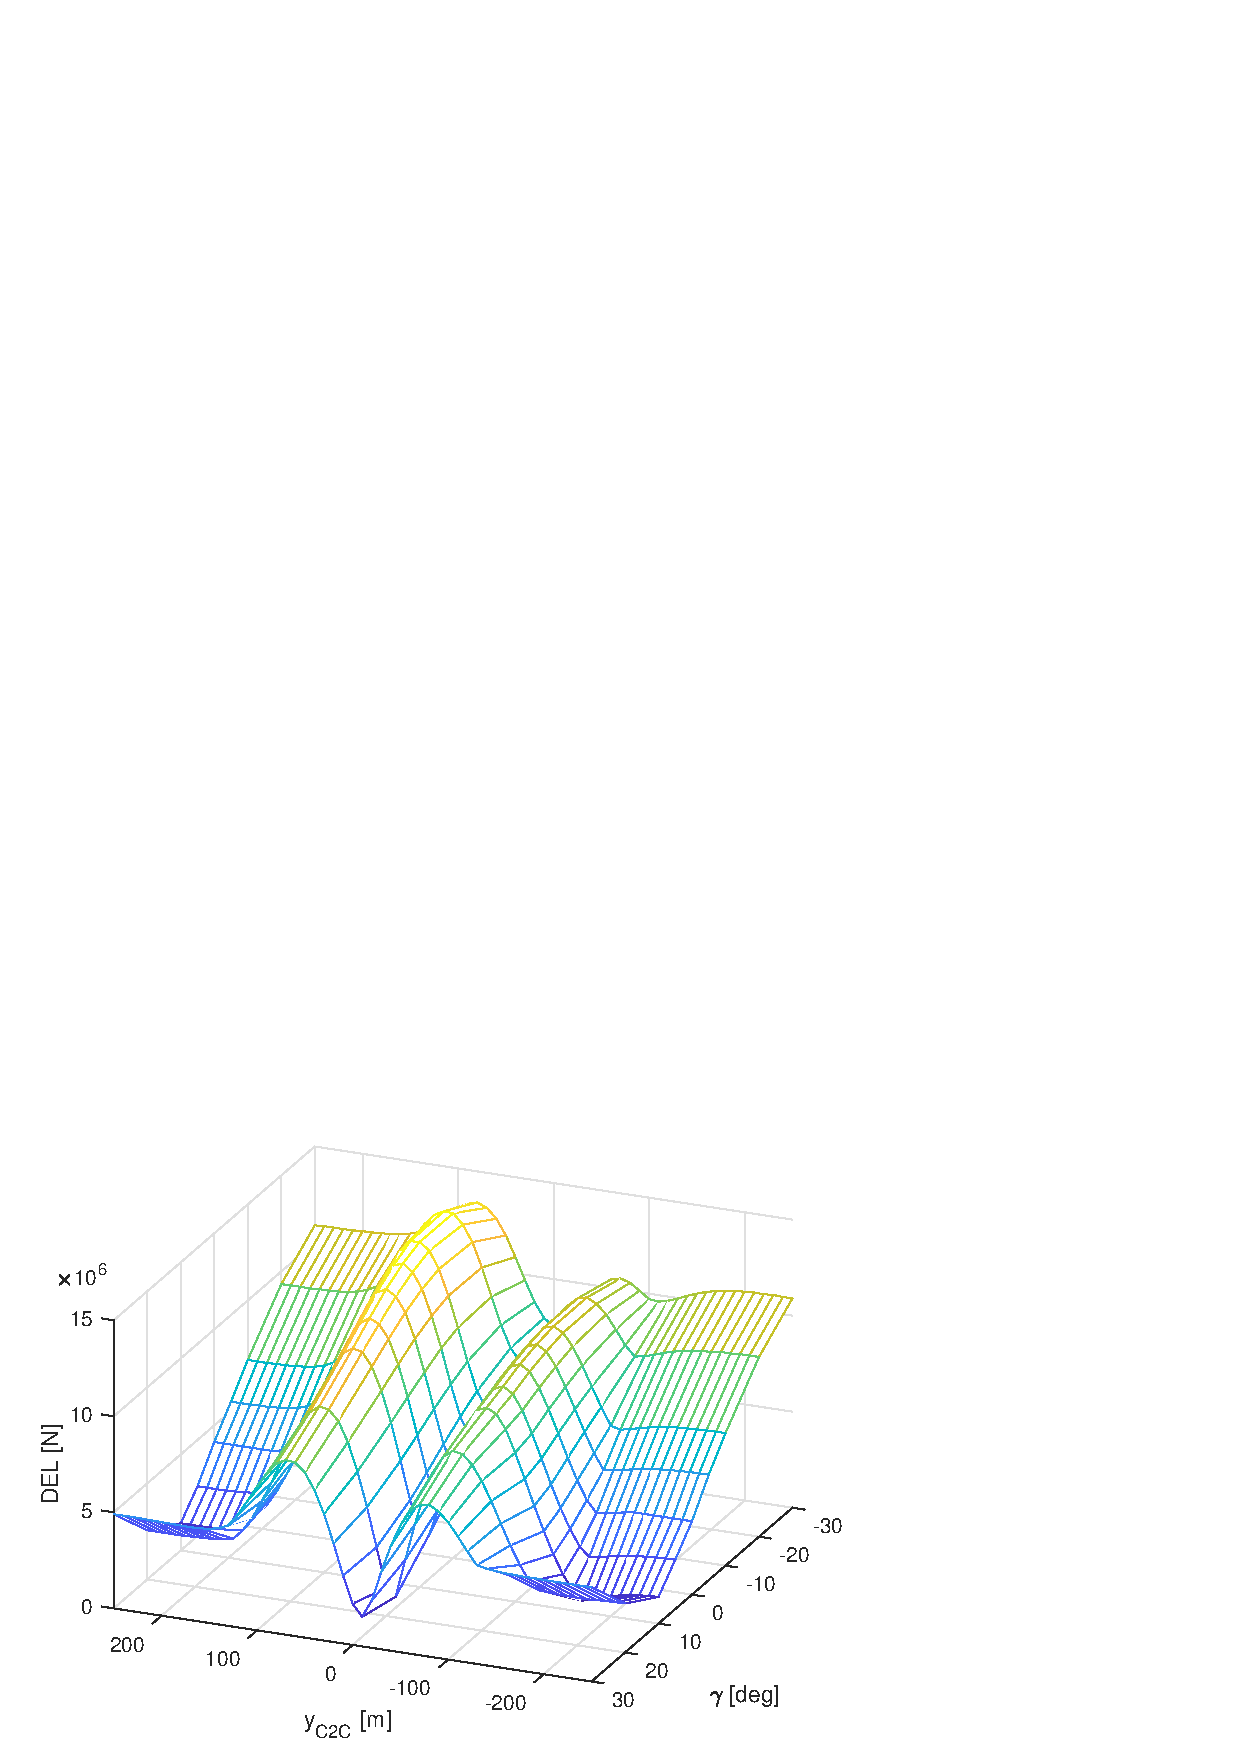
\includegraphics[width=\linewidth]{./Figures/LUTslice_Dw230_Ufs8.jpg}
	\caption{Slice of the LUT with a $D_{wake}$ of 230m and a $U_{fs}$ of 8m/s }
	\label{fig:LUTslice}
\end{figure}

\subsection{Optimization}
The optimization script is run on a set of nine wind turbines which are place in a 3-by-3 grid. As a reference 'greedy control' is used. To determine the maximum power the nine wind turbines can deliver an optimization is executed taking only power into account. See table \ref{tab:reference} for the power and DEL values for both these situations. \newline
To show the optimization script in action five cases are evaluated. Each case has its reference power $P_{ref}$ set as a percentage of the maximum power. In figure \ref{fig:optimization90pct} power and DEL values during optimization with a reference power of 90\% are shown. Figure \ref{fig:config90pct} shows the final turbine configuration for this optimization run. \newline
Figure \ref{fig:optimizationTrends} shows the DEL values for different reference powers.


\begin{table}[h]
	\caption{Power and DEL values for greedy control and power-only optimization}
	\centering
	\label{tab:reference}
	\begin{tabular}{lccc}
		\hline
		& Greedy control & Power-only \\ 
		\hline
		Power [MW] & 12.42 & 13.22 \\
		DEL value [-] & 5.94E7 & - \\
		\hline
	\end{tabular}
\end{table}

\begin{figure}
	\includegraphics[width=\linewidth]{./Figures/{Configuration_Pref11.9}.jpg}
	\caption{Turbine configuration after optimization with $P_{ref}$ at 90\% }
	\label{fig:config90pct}
\end{figure}

\begin{figure}
	\includegraphics[width=\linewidth]{./Figures/{Optimization_Pref11.9}.jpg}
	\caption{Loads and power during optimization with $P_{ref}$ at 90\% }
	\label{fig:optimization90pct}
\end{figure}

\begin{figure}
	\includegraphics[width=\linewidth]{./Figures/trendPlot.jpg}
	\caption{DEL values for different $P_{ref}$}
	\label{fig:optimizationTrends}
\end{figure}
         